\subsection{Functions of Bounded Variation}
\begin{frame}[noframenumbering]{Table of Contents}
  \tableofcontents[currentsection, currentsubsection]
\end{frame}

\begin{frame}
  Let $U$ be an open subset of $\Rbb^d$. A function $v\in L^1(U)$ is a function
  of bounded variation iff
  \begin{align*}
    |v|_{\BV(U)}
    \coloneqq
    \sup_{\substack{\phi\in C^1_C(U;\Rbb^d)\\
    \Vert\phi\Vert_{L^\infty(U)}\leq 1}}\int_U v\Div (\phi)\dx
    <
    \infty.
  \end{align*}
  The space of all such functions is denoted by $\BV(U)$.
  \pause
  It is a Banach space equipped with the norm $\Vert \bullet
  \Vert_{\BV(U)} \coloneqq \Vert \bullet\Vert_{L^1(U)} + |\bullet|_{\BV(U)}$.

  \pause
  \medskip
  We have $W^{1,1}(\Omega)\subset\BV(\Omega)$ with $\Vert v\Vert_{\BV(\Omega)}=
  \Vert v\Vert_{W^{1,1}(\Omega)}$ for all $v\in W^{1,1}(\Omega)$.
\end{frame}

\begin{frame}
  \fullcite{ABM14}

  \bigskip

  \fullcite{EG92}
\end{frame}

\subsection{Rudin-Osher-Fatemi Model Problem}
\begin{frame}[noframenumbering]{Table of Contents}
  \tableofcontents[currentsection, currentsubsection]
\end{frame}

\begin{frame}
  Let $\Omega\subset\Rbb^2$ be a bounded polygonal Lipschitz domain.
  \begin{block}{Rudin-Osher-Fatemi (ROF) model problem}
    For a parameter $\alpha\in \Rbb_+$ and an input signal $g\in L^2(\Omega)$
    minimize the functional
    \begin{align*}
      I(v)
      \coloneqq 
      {\color<4>{red}{|v|_{\BV(\Omega)}}}
      +\frac{\alpha}{2}
      {\color<3>{red}{\Vert v-g\Vert_{L^2(\Omega)}^2}}
    \end{align*}
    amongst all $v\in\BV(\Omega)\cap L^2(\Omega)$.
  \end{block}

  \bigskip
  \pause
  \fullcite{ROF92}
\end{frame}

\begin{frame}
  \begin{figure}[!ht]
    \centering
    \begin{subfigure}{.4\linewidth}
      \caption*{Original picture$^0$}
      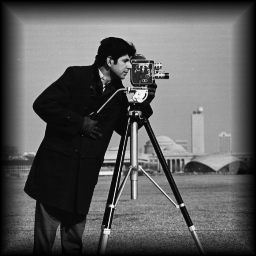
\includegraphics[width=\linewidth]
        {pictures/recap/denoiseExample/cameraman.png}
    \end{subfigure}
    \quad
    \uncover<2->{
    \begin{subfigure}{.4\linewidth}
      \caption*{Input signal}
      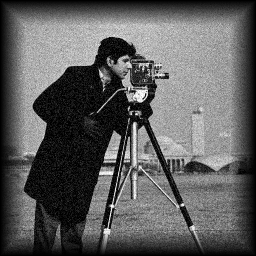
\includegraphics[width=\linewidth]
        {pictures/recap/denoiseExample/snr20.png}
    \end{subfigure}}
  \end{figure}
  \footnotetext{
  \url{https://homepages.cae.wisc.edu/~ece533/images/cameraman.tif}}
\uncover<2->{The input signal was created by adding AWGN with a SNR of 20 to
the original picture.}
\end{frame}

\begin{frame}
  \vspace{-4mm}
    \begin{align*}
      I(v)
      \coloneqq 
      {\color<3>{red}{|v|_{\BV(\Omega)}}}
      +\frac{\alpha}{2}
      {\color<2>{red}{\Vert v-g\Vert_{L^2(\Omega)}^2}}
    \end{align*}
  \vspace{-7mm}
  \begin{figure}[!ht]
    \centering
    \begin{subfigure}{.3\linewidth}
      \caption*{Original picture}
      \vspace{-2mm}
      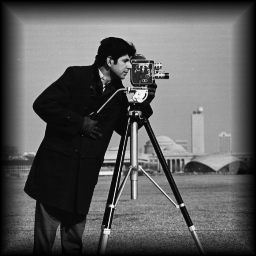
\includegraphics[width=\linewidth]
        {pictures/recap/denoiseExample/cameraman.png}
    \end{subfigure}
    \quad
    \begin{subfigure}{.3\linewidth}
      \caption*{Input signal}
      \vspace{-2mm}
      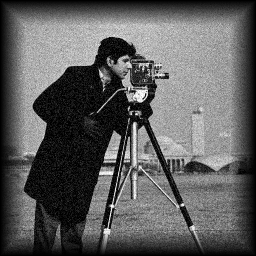
\includegraphics[width=\linewidth]
        {pictures/recap/denoiseExample/snr20.png}
    \end{subfigure}
  
    \vspace{3mm}
    \uncover<3->{
    \begin{subfigure}{.3\linewidth}
      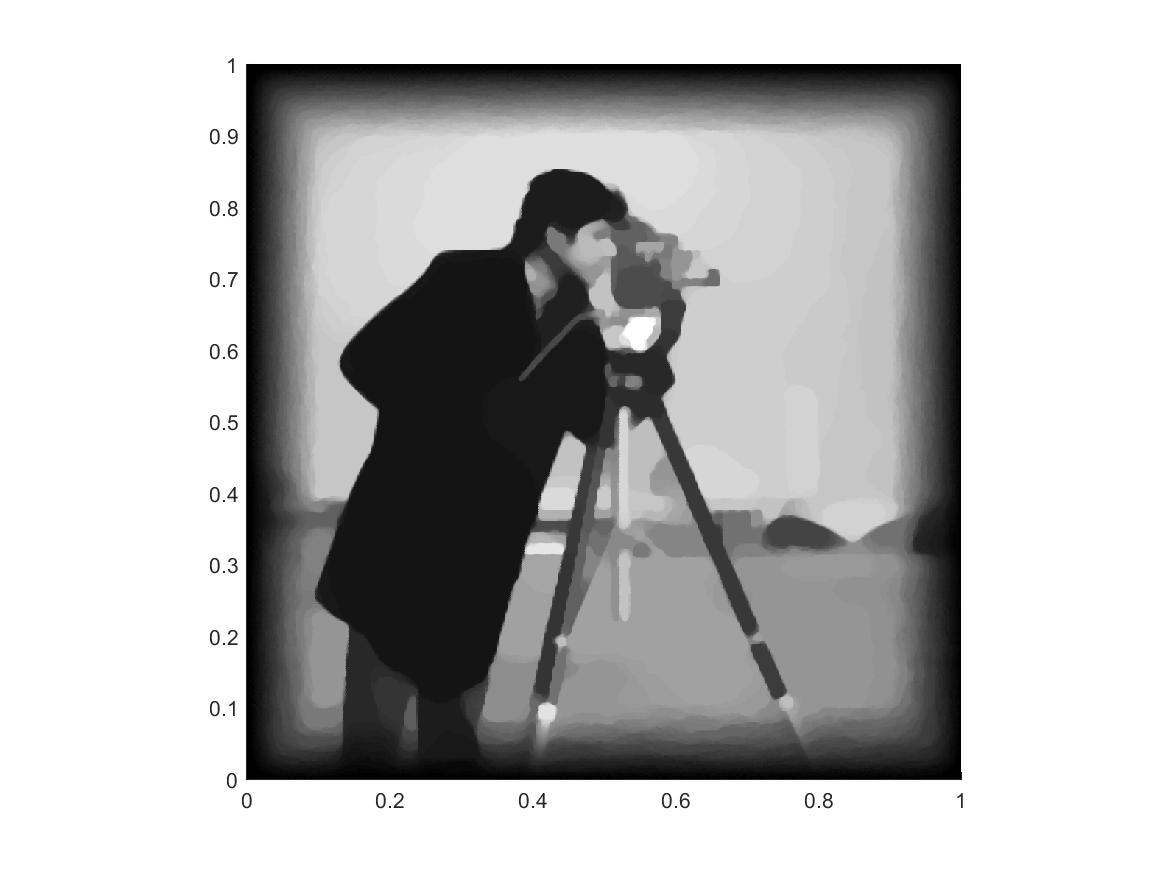
\includegraphics[trim = 60 20 60 20, clip, width=\linewidth]
        {pictures/recap/denoiseExample/alpha1e3.png}
      \caption*{$\alpha=10^3$}
    \end{subfigure}}
    \uncover<4->{
    \begin{subfigure}{.3\linewidth}
      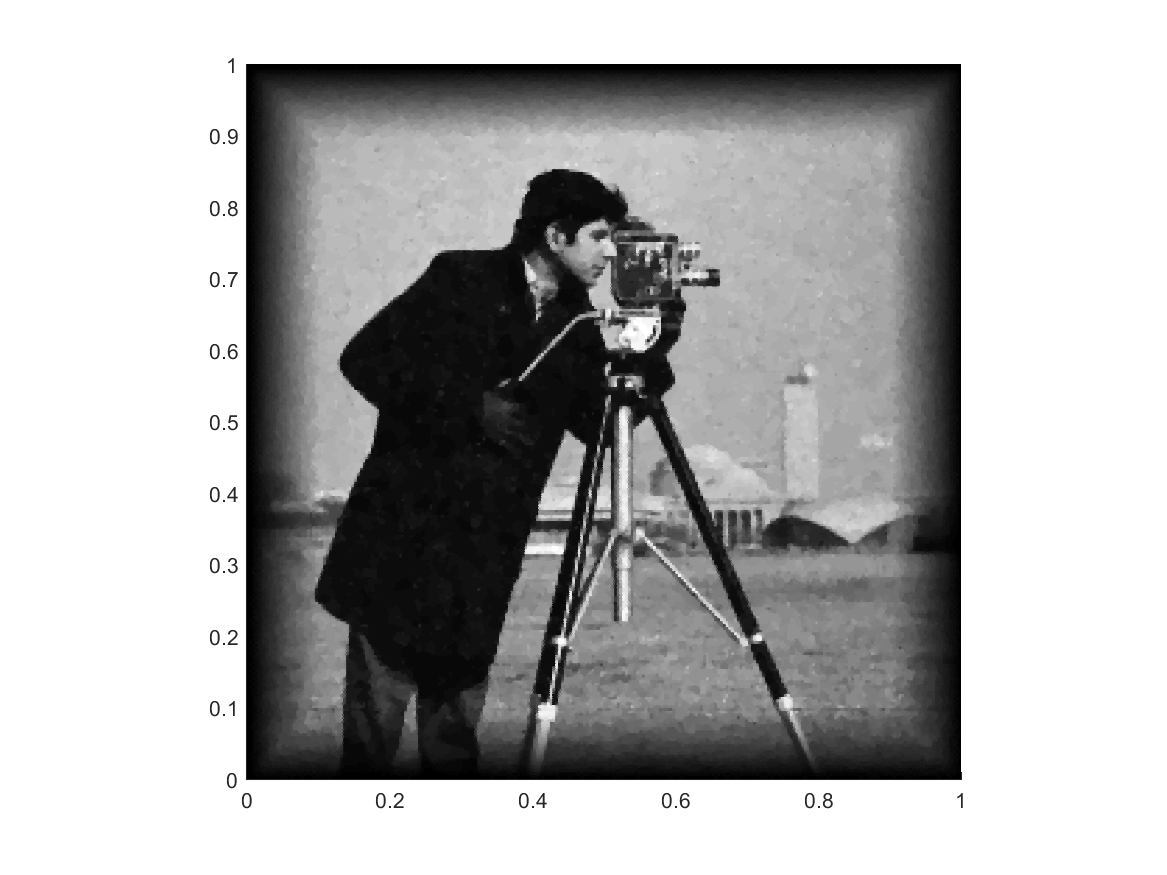
\includegraphics[trim = 60 20 60 20, clip, width=\linewidth]
        {pictures/recap/denoiseExample/alpha1e4.png}
      \caption*{$\alpha=10^4$}
    \end{subfigure}}
    \uncover<2->{
    \begin{subfigure}{.3\linewidth}
      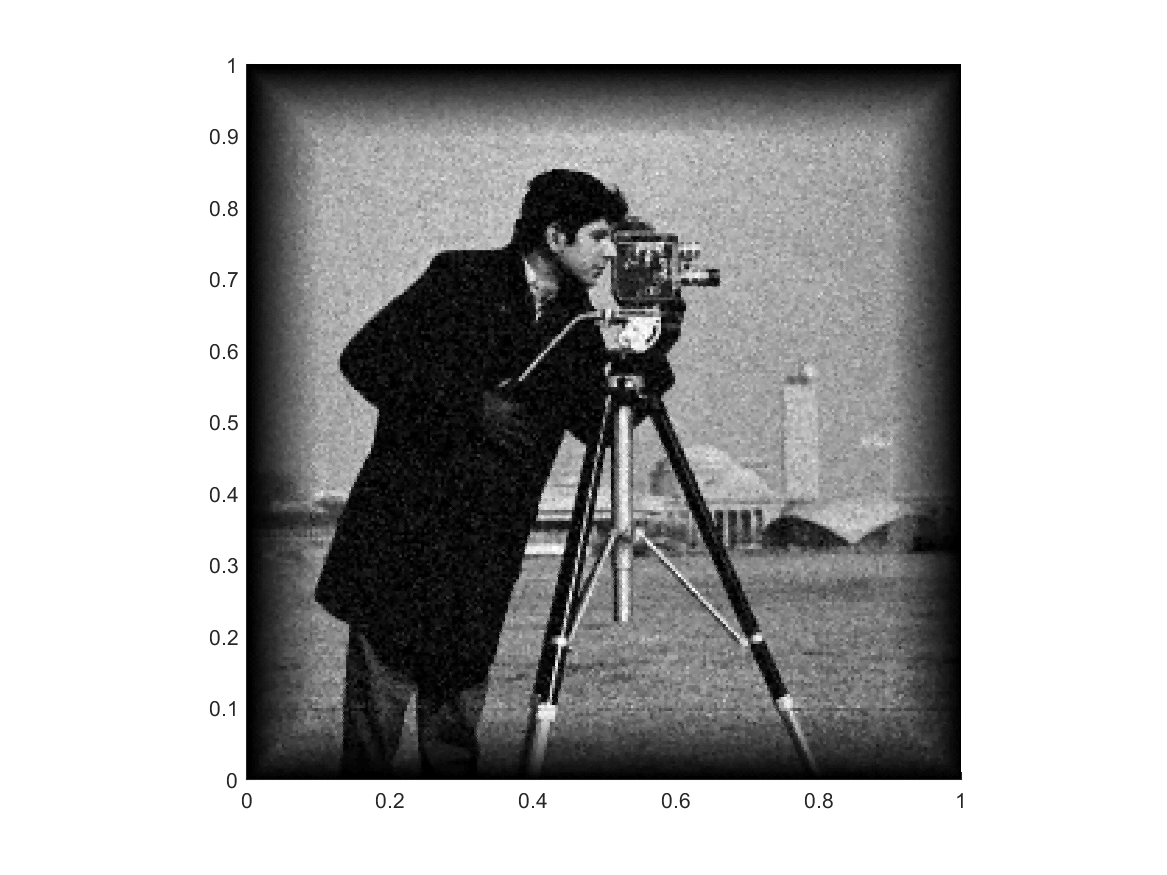
\includegraphics[trim = 60 20 60 20, clip, width=\linewidth]
        {pictures/recap/denoiseExample/alpha1e5.png}
      \caption*{$\alpha=10^5$}
    \end{subfigure}}
  \end{figure}
\end{frame}

\begin{frame}
  \fullcite{Get12}
\end{frame}

\subsection{Continuous Problem}
\begin{frame}[noframenumbering]{Table of Contents}
  \tableofcontents[currentsection, currentsubsection]
\end{frame}

\begin{frame}
  \begin{block}{Continuous problem}
    For a parameter $\alpha\in \Rbb_+$ and an input signal $f\in L^2(\Omega)$
    minimize the functional
    \begin{align*}\label{eq:continuousProblem}
      E(v)\coloneqq \frac{\alpha}{2}\Vert v\Vert^2 
      + |v|_{\BV(\Omega)} 
      + {\color<2>{red}{\Vert v\Vert_{L^1(\partial\Omega)}}}
      - \int_\Omega fv\dx
    \end{align*}
    amongst all $v\in\BV(\Omega)\cap L^2(\Omega)$.
  \end{block}

  \bigskip
  \uncover<3->{
  For $f=\alpha g$ the functional $E$ has the same minimizers as
  \begin{align*}
    I(v)
    = 
    |v|_{\BV(\Omega)}
    +\frac{\alpha}{2}
    \Vert v-g\Vert_{L^2(\Omega)}^2
  \end{align*}
  in $\left\{v\in\BV(\Omega)\cap L^2(\Omega) \mid \Vert
  v\Vert_{L^1(\partial\Omega)}=0\right\}$.}
\end{frame}

\begin{frame}
  \begin{theorem}[Existence and uniqueness]
    There exists a unique minimizer $u\in\BV(\Omega)\cap L^2(\Omega)$ for
    $E=\frac{\alpha}{2}\Vert v\Vert^2 
      + {\color<2>{red}{|v|_{\BV(\Omega)} 
      + \Vert v\Vert_{L^1(\partial\Omega)}}}
      - \int_\Omega fv\dx$ in 
     $v\in\BV(\Omega)\cap L^2(\Omega)$.
  \end{theorem}

  \pause
  \medskip
  \begin{lemma}
    Let $v\in\BV(\Omega)$.
    For all $x\in\Rbb^d$, define
    \begin{align*}
      \tilde{v}(x)\coloneqq
      \begin{cases}
        v(x)  &\text{if } x\in\Omega,\\
        0     &\text{if } x\in\Rbb^d\setminus\overline\Omega.
      \end{cases} 
    \end{align*}
    Then $\tilde{v}\in\BV\!\left(\Rbb^d\right)$ and
    $\left|\tilde{v}\right|_{\BV\!\left(\Rbb^d\right)}
    = |v|_{\BV(\Omega)}+\Vert v\Vert_{L^1(\partial\Omega)}$.
  \end{lemma}
\end{frame}


\begin{frame}
  Let $U$ be an open subset of $\Rbb^d$.

  \begin{definition}[Weak convergence in $\BV(U)$]
    Let $(v_n)_{n\in\Nbb}\subset \BV(U)$ and $v\in \BV(U)$ with
    $v_n\rightarrow v$ in $L^1(U)$ as $n\rightarrow\infty$.
    Then $(v_n)_{n\in\Nbb}$ converges weakly to $v$ in $\BV(U)$ iff,
    for all $\phi\in C_0(U;\Rbb^d)$, it holds
    \begin{align*}
      \int_U v_n\Div(\phi)\dx\rightarrow \int_U v\Div(\phi)\dx 
      \quad\text{as } n\to\infty. 
    \end{align*}
    We write $v_n\rightharpoonup v$ as $n\to\infty$.
  \end{definition}
\end{frame}

\begin{frame}
  \begin{theorem}
    Let $v\in L^1(U)$ and $(v_n)_{n\in\Nbb}\subset\BV(U)$ with
    $\sup_{n\in\Nbb}|v_n|_{\BV(U)}< \infty$ and
    $v_n\rightarrow v$ in $L^1(U)$ as $n\rightarrow\infty$.
    Then $v\in\BV(U)$ and $|v|_{\BV(U)}\leq
    \liminf_{n\rightarrow\infty}|v_n|_{\BV(U)}.$
    Furthermore, $v_n\rightharpoonup v$ in $\BV(U)$.
  \end{theorem}

  \pause
  \medskip
  Let $U$ be a bounded Lipschitz domain.
  
  \begin{theorem}[\protect{\cite[S. 176, Theorem 4]{EG92}}]
    \label{thm:l1ConvergentSubsequence}
    Let $(v_n)_{n\in\Nbb}\subset \BV(U)$ be bounded. Then
    there exists some subsequence $(v_{n_k})_{k\in\Nbb}$ of
    $(v_n)_{n\in\Nbb}$ and $v\in\BV(U)$ such that
    $v_{n_k}\to v$ in $L^1(U)$ as $k\to \infty$.
  \end{theorem}
\end{frame}

\begin{frame}
  \begin{block}{Stability}
    Let $f_1,f_2\in L^2(\Omega)$.
    For $\ell\in\{1,2\}$, let $u_\ell\in \BV(\Omega)\cap L^2(\Omega)$ minimize
    \begin{align*}
      E_\ell
      \coloneqq 
      {\color<3>{red}{\frac{\alpha}{2}\Vert v\Vert^2}}
      + {\color<4>{red}{|v|_{\BV(\Omega)} 
      + \Vert v\Vert_{L^1(\partial\Omega)} }}
      {\color<3>{red}{- \int_\Omega f_\ell v\dx}}
    \end{align*}
    amongst all $v\in\BV(\Omega)\cap L^2(\Omega)$.
    Then
    \begin{align*}
      \Vert u_1 - u_2\Vert 
      \leq\frac{1}{\alpha}\Vert f_1-f_2\Vert.
    \end{align*}
  \end{block}

  \medskip
  \pause
  \fullcite[Chapter 10]{Bar15}.

\end{frame}

\subsection{Discrete Problem}
\begin{frame}[noframenumbering]{Table of Contents}
  \tableofcontents[currentsection, currentsubsection]
\end{frame}

\begin{frame}
  nochmal Existenz und Eindeutigkeitsaussagen zeigen und gaaaanz grob 
  beschreiben, wie die bewiesen werden
\end{frame}

\subsection{Discrete Problem continues}
\begin{frame}[noframenumbering]{Table of Contents}
  \tableofcontents[currentsection, currentsubsection]
\end{frame}

\begin{frame}
  vielleicht in eigener Section: noch die Aussagen aus der Arbeit verarbeiten,
  die über Existenz und Eindeutigkeit hinausgehen
\end{frame}


\begin{frame}
  \fullcite[Chapter 10, p. 297-319]{Bar15}
\end{frame}

\begin{frame}{Properties of $\BV(\Omega)$}
\end{frame}

\begin{frame}{Notions of convergence on $\BV(\Omega)$}
  Let $(v_n)_{n\in\Nbb}\subset \BV(\Omega)$ and $v\in \BV(\Omega)$ such that
  $v_n\rightarrow v$ in $L^1(\Omega)$ as $n\rightarrow\infty$.
  \pause
  \begin{itemize}
    \item[(i)]
      $(v_n)_{n\in\Nbb}$ converges intermediately or strictly to $v$
      if $|v_n|_{\BV(\Omega)}\rightarrow |v|_{\BV(\Omega)}$ as
      $n\rightarrow\infty$.
      \pause
    \item[(ii)] $(v_n)_{n\in\Nbb}$ converges weakly to
      $v$ if
      $\langle Dv_n,\phi\rangle\rightarrow \langle Dv,\phi\rangle$ 
      for all $\phi\in C_0(\Omega;\Rbb^n)$ as 
      $n\rightarrow\infty$.
  \end{itemize}
\end{frame}

\begin{frame}{Further Properties of $\BV(\Omega)$}
  $C^\infty(\overline\Omega)$ and $C^\infty(\Omega)\cap\BV(\Omega)$ are dense
  in $\BV(\Omega)$ with respect to intermediate convergence.
  
  \pause
  \bigskip

  The embedding $\BV(\Omega)\to L^p(\Omega)$ is continuous for
  $1\leq p\leq n/(n-1)$ and compact for $1\leq p< n/(n-1)$.
  
  \pause
  \bigskip

  There exists a linear operator $T:\BV(\Omega)\to L^1(\partial\Omega)$
  such that $T(v) = v|_{\partial\Omega}$ for all $v\in\BV(\Omega)\cap
  C(\overline\Omega)$.

  $T$ is continuous with respect to intermediate convergence in $\BV(\Omega)$
  but not with respect to weak convergence in $\BV(\Omega)$. 
\end{frame}

